\documentclass[10pt]{article}
\usepackage{amsmath}
\usepackage{mathtools}
\DeclarePairedDelimiter{\abs}{\lvert}{\rvert}
\usepackage[hidelinks]{hyperref}
\usepackage{amssymb}
\usepackage{tikz}
\usepackage{caption}
\usepackage{graphicx}
\usepackage[T1]{fontenc}
\graphicspath{{.}}
\usepackage{listings}
\usepackage{verbatim}
\usepackage{floatrow}
\usepackage{bigints}
\lstset{
language=[LaTeX]TeX,
backgroundcolor=\color{gray!25},
basicstyle=\ttfamily,
columns=flexible,
breaklines=true
}
\captionsetup{labelsep=colon,justification=centering,singlelinecheck=off}
\reversemarginpar
\usepackage[paper=a4paper,
            %includefoot, % Uncomment to put page number above margin
            marginparwidth=10mm,      % Length of section titles
            marginparsep=0.8mm,       % Space between titles and text
            margin=11mm,              % 25mm margins
            includemp]{geometry}

\begin{document}
\section*{}
\begin{flushleft}
Name: Krishna Chaitanya Sripada\\
\end{flushleft}
\section*{Ans 1}
\begin{flushleft}
Expected adjacency matrix M = $\mathbb{E}$[A] computed over all possible realizations of $\mathcal{B}$ is calculated as follows:\\
\vspace{0.5em}
$\mathbb{E}$[B(p)] = 1 $\times$ p + 0 $\times$ (1 - p) = p and $\mathbb{E}$[B(q)] = 1 $\times$ q + 0 $\times$ (1 - q) = q.\\
\vspace{0.5em}
Given $T$ is a random permutation matrix,\\
\vspace{0.5em}
$$ T = 
\begin{bmatrix} 
1 & \hdots & 0 & 0 & \hdots & 0\\
\vdots & & \vdots & \vdots & & \vdots\\
\vdots & & \vdots & \vdots & & \vdots\\
0 & \hdots & 0 & 1 & \hdots & 0\\
0 & \hdots & 1 & 0 & \hdots & 0\\ 
\vdots & & \vdots & \vdots & & \vdots\\
\vdots & & \vdots & \vdots & & \vdots\\
0 & \hdots & 0 & 0 & \hdots & 1\\
\end{bmatrix}
$$
\vspace{0.5em}
$$ T^{T} = 
\begin{bmatrix} 
1 & \hdots & 0 & 0 & \hdots & 0\\
\vdots & & \vdots & \vdots & & \vdots\\
\vdots & & \vdots & \vdots & & \vdots\\
0 & \hdots & 0 & 1 & \hdots & 0\\
0 & \hdots & 1 & 0 & \hdots & 0\\ 
\vdots & & \vdots & \vdots & & \vdots\\
\vdots & & \vdots & \vdots & & \vdots\\
0 & \hdots & 0 & 0 & \hdots & 1
\end{bmatrix}
$$
Therefore, $A = T\mathcal{B}T^{T} = \mathcal{B}$. By substituting the Bernoulli random variable values, we get, \\
\vspace{0.5em}
$$ M = 
\begin{bmatrix} 
p & \hdots & p & q & \hdots & q\\
\vdots & & \vdots & \vdots & & \vdots\\
\vdots & & \vdots & \vdots & & \vdots\\
p & \hdots & p & q & \hdots & q\\
q & \hdots & q & p & \hdots & p\\ 
\vdots & & \vdots & \vdots & & \vdots\\
\vdots & & \vdots & \vdots & & \vdots\\
q & \hdots & q & p & \hdots & p
\end{bmatrix}
$$
\end{flushleft}
\section*{Ans 2}
\begin{flushleft}
The degree matrix is defined as the diagonal matrix with entries $d_{i} = \sum_{j=1}^{n} A_{i,j} = \frac{1}{2} (n \times p + n \times q) = \frac{n}{2}(p+q)$. Therefore, the expected degree matrix is,\\
\vspace{0.5em}
$$ \mathbb{E}[D] = 
\begin{bmatrix} 
\frac{n}{2}(p+q) & \hdots & 0 & 0 & \hdots & 0\\
\vdots & & \vdots & \vdots & & \vdots\\
\vdots & & \vdots & \vdots & & \vdots\\
0 & \hdots & \frac{n}{2}(p+q) & 0 & \hdots & 0\\
0 & \hdots & 0 & \frac{n}{2}(q+p) & \hdots & 0\\ 
\vdots & & \vdots & \vdots & & \vdots\\
\vdots & & \vdots & \vdots & & \vdots\\
0 & \hdots & 0 & 0 & \hdots & \frac{n}{2}(q+p)
\end{bmatrix}
$$
\end{flushleft}
\section*{Ans 3}
\begin{flushleft}
If $w_{1}$ is an eigenvector of M, then $Mw_{1} = \lambda w_{1}$. Given $w_{1} = \frac{1}{\sqrt n} \mathcal{I}$ where $\mathcal{I}$ =1 $\forall$ i = 1, $\hdots$ , n.\\
\vspace{0.5em}
$$ w_{1} = 
\begin{bmatrix}
\frac{1}{\sqrt n}\\
\vdots\\
\vdots\\
\frac{1}{\sqrt n}\\
\frac{1}{\sqrt n}\\
\vdots\\
\vdots\\
\frac{1}{\sqrt n}
\end{bmatrix}
$$
Then, \\
\vspace{0.5em}
$$ Mw_{1} = 
\begin{bmatrix}
\frac{n}{2 \sqrt n} (p+q)\\
\vdots\\
\vdots\\
\frac{n}{2 \sqrt n} (p+q)\\
\frac{n}{2 \sqrt n} (p+q)\\
\vdots\\
\vdots\\
\frac{n}{2 \sqrt n} (p+q)
\end{bmatrix}
$$
Since $Mw_{1}$ can be expressed as $\lambda w_{1}$, we can say that $w_{1}$ is an eigenvector of M. \\
\vspace{0.5em}
Also the eigenvalue $\mu_{1}$ is given by,\\
\vspace{0.5em}
$$ Mw_{1} = 
\begin{bmatrix}
\frac{n}{2 \sqrt n} (p+q)\\
\vdots\\
\vdots\\
\frac{n}{2 \sqrt n} (p+q)\\
\frac{n}{2 \sqrt n} (p+q)\\
\vdots\\
\vdots\\
\frac{n}{2 \sqrt n} (p+q)
\end{bmatrix}
= \lambda w_{1}
= \begin{bmatrix}
\frac{\lambda}{\sqrt n}\\
\vdots\\
\vdots\\
\frac{\lambda}{\sqrt n}\\
\frac{\lambda}{\sqrt n}\\
\vdots\\
\vdots\\
\frac{\lambda}{\sqrt n}
\end{bmatrix}
$$
Therefore, we have,\\
\vspace{0.5em}
$\frac{n}{2 \sqrt n} (p+q) = \frac{\lambda}{\sqrt n}$\\
\vspace{0.5em}
$\lambda = \frac{n}{2} (p+q)$
\end{flushleft}
\section*{Ans 4}
\begin{flushleft}
To prove that $w_{2}$ is an eigenvector of M. We should be able to prove that $Mw_{2} = \lambda w_{2}$. \\
\vspace{0.5em}
Let $$ w_{2} = 
\begin{bmatrix}
\frac{1}{\sqrt n}\\
\vdots\\
\vdots\\
\frac{1}{\sqrt n}\\
\frac{-1}{\sqrt n}\\
\vdots\\
\vdots\\
\frac{-1}{\sqrt n}
\end{bmatrix}
$$
Then, \\
\vspace{0.5em}
$$ Mw_{2} = 
\begin{bmatrix}
\frac{n}{2 \sqrt n} (p-q)\\
\vdots\\
\vdots\\
\frac{n}{2 \sqrt n} (p-q)\\
\frac{n}{2 \sqrt n} (q-p)\\
\vdots\\
\vdots\\
\frac{n}{2 \sqrt n} (q-p)
\end{bmatrix}
= 
\begin{bmatrix}
\frac{n}{2 \sqrt n} (p-q)\\
\vdots\\
\vdots\\
\frac{n}{2 \sqrt n} (p-q)\\
\frac{-n}{2 \sqrt n} (p-q)\\
\vdots\\
\vdots\\
\frac{-n}{2 \sqrt n} (p-q)
\end{bmatrix}
$$
Since $Mw_{2}$ can be expressed as $\lambda w_{2}$, we can say that $w_{2}$ is an eigenvector of M. \\
\vspace{0.5em}
Also the eigenvalue $\mu_{2}$ is given by,\\
\vspace{0.5em}
$$ Mw_{2} = 
\begin{bmatrix}
\frac{n}{2 \sqrt n} (p-q)\\
\vdots\\
\vdots\\
\frac{n}{2 \sqrt n} (p-q)\\
\frac{-n}{2 \sqrt n} (p-q)\\
\vdots\\
\vdots\\
\frac{-n}{2 \sqrt n} (p-q)
\end{bmatrix}
= \lambda w_{2}
= \begin{bmatrix}
\frac{\lambda}{\sqrt n}\\
\vdots\\
\vdots\\
\frac{\lambda}{\sqrt n}\\
\frac{-\lambda}{\sqrt n}\\
\vdots\\
\vdots\\
\frac{-\lambda}{\sqrt n}
\end{bmatrix}
$$
Therefore, we have,\\
\vspace{0.5em}
$\frac{n}{2 \sqrt n} (p-q) = \frac{\lambda}{\sqrt n}$\\
\vspace{0.5em}
$\lambda = \frac{n}{2} (p-q)$
\end{flushleft}
\section*{Ans 5}
\begin{figure}[!htb]
    \begin{floatrow}
         \ffigbox{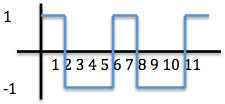
\includegraphics[scale = 0.8]{w3.png}}{\caption{Graph of $w_{3}$}\label{w3}}
         \ffigbox{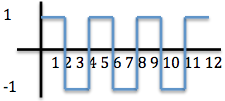
\includegraphics[scale = 0.8]{w4.png}}{\caption{Graph of $w_{4}$}\label{w4}}
    \end{floatrow}
\end{figure}
\section*{Ans 6}
\begin{flushleft}
We need to prove that $Mw_{3} = 0$ and $Mw_{4}=0$. We have 
$$ w_{3} = 
\begin{bmatrix}
\frac{1}{\sqrt n}\\
\vdots\\
\frac{1}{\sqrt n}\\
\frac{-1}{\sqrt n}\\
\vdots\\
\frac{-1}{\sqrt n}\\
\vdots\\
\frac{1}{\sqrt n}\\
\vdots\\
\frac{1}{\sqrt n}
\end{bmatrix}
$$
Therefore, \\
$$ Mw_{3} = 
\begin{bmatrix}
\frac{n}{4 \sqrt n} (p+q) - \frac{n}{2 \sqrt n} (p+q) + \frac{n}{4 \sqrt n} (p+q)\\
\vdots\\
\vdots\\
\frac{n}{4 \sqrt n} (p+q) - \frac{n}{2 \sqrt n} (p+q) + \frac{n}{4 \sqrt n} (p+q)\\
\frac{n}{4 \sqrt n} (p+q) - \frac{n}{2 \sqrt n} (p+q) + \frac{n}{4 \sqrt n} (p+q)\\
\vdots\\
\vdots\\
\frac{n}{4 \sqrt n} (p+q) - \frac{n}{2 \sqrt n} (p+q) + \frac{n}{4 \sqrt n} (p+q)
\end{bmatrix}
= \begin{bmatrix}
0\\
\vdots\\
\vdots\\
0\\
0\\
\vdots\\
\vdots\\
0
\end{bmatrix}
$$
$$ w_{4} = 
\begin{bmatrix}
\frac{1}{\sqrt n}\\
\vdots\\
\frac{-1}{\sqrt n}\\
\frac{1}{\sqrt n}\\
\vdots\\
\frac{1}{\sqrt n}\\
\vdots\\
\frac{-1}{\sqrt n}\\
\vdots\\
\frac{-1}{\sqrt n}
\end{bmatrix}
$$
Therefore, \\
$$ Mw_{4} = 
\begin{bmatrix}
\frac{n}{4 \sqrt n} (p) - \frac{n}{4 \sqrt n} (q) + \frac{n}{4 \sqrt n} (q) - \frac{n}{4 \sqrt n} (p)\\
\vdots\\
\vdots\\
\frac{n}{4 \sqrt n} (p) - \frac{n}{4 \sqrt n} (q) + \frac{n}{4 \sqrt n} (q) - \frac{n}{4 \sqrt n} (p)\\
\frac{n}{4 \sqrt n} (p) - \frac{n}{4 \sqrt n} (q) + \frac{n}{4 \sqrt n} (q) - \frac{n}{4 \sqrt n} (p)\\
\vdots\\
\vdots\\
\frac{n}{4 \sqrt n} (p) - \frac{n}{4 \sqrt n} (q) + \frac{n}{4 \sqrt n} (q) - \frac{n}{4 \sqrt n} (p)
\end{bmatrix}
= \begin{bmatrix}
0\\
\vdots\\
\vdots\\
0\\
0\\
\vdots\\
\vdots\\
0
\end{bmatrix}
$$
\end{flushleft}
\section*{Ans 7}
\begin{flushleft}
We have $\mu_{1} = \frac{n (p+q)}{2}$ and $\mu_{2} = \frac{n (p-q)}{2}$. To prove that $M = \mu_{1}w_{1}w_{1}^{T} + \mu_{2}w_{2}w_{2}^{T}$, lets multiply the corresponding matrices. By doing so, we get,\\
$$
\begin{bmatrix}
\frac{n (p+q)}{2\sqrt n}\\
\vdots\\
\vdots\\
\frac{n (p+q)}{2\sqrt n}\\
\frac{n (p+q)}{2\sqrt n}\\
\vdots\\
\vdots\\
\frac{n (p+q)}{2\sqrt n}\\
\end{bmatrix}
\begin{bmatrix}
\frac{1}{\sqrt n} &\hdots &\hdots &\frac{1}{\sqrt n} &\frac{1}{\sqrt n} &\hdots &\hdots & \frac{1}{\sqrt n}
\end{bmatrix}
+ 
\begin{bmatrix}
\frac{n (p-q)}{2\sqrt n}\\
\vdots\\
\vdots\\
\frac{n (p-q)}{2\sqrt n}\\
\frac{n (q-p)}{2\sqrt n}\\
\vdots\\
\vdots\\
\frac{n (q-p)}{2\sqrt n}\\
\end{bmatrix}
\begin{bmatrix}
\frac{1}{\sqrt n} &\hdots &\hdots &\frac{1}{\sqrt n} &\frac{-1}{\sqrt n} &\hdots &\hdots & \frac{-1}{\sqrt n}
\end{bmatrix}
$$
$$
\begin{bmatrix} 
\frac{p+q}{2} & \hdots & \frac{p+q}{2} & \frac{q+p}{2}& \hdots & \frac{q+p}{2}\\
\vdots & & \vdots & \vdots & & \vdots\\
\vdots & & \vdots & \vdots & & \vdots\\
\frac{p+q}{2} & \hdots & \frac{p+q}{2} & \frac{q+p}{2} & \hdots & \frac{q+p}{2}\\
\frac{q+p}{2} & \hdots & \frac{q+p}{2} & \frac{p+q}{2} & \hdots & \frac{p+q}{2}\\ 
\vdots & & \vdots & \vdots & & \vdots\\
\vdots & & \vdots & \vdots & & \vdots\\
\frac{q+p}{2} & \hdots & \frac{q+p}{2} & \frac{p+q}{2} & \hdots & \frac{p+q}{2}
\end{bmatrix}
+
\begin{bmatrix} 
\frac{p-q}{2} & \hdots & \frac{p-q}{2} & \frac{q-p}{2}& \hdots & \frac{q-p}{2}\\
\vdots & & \vdots & \vdots & & \vdots\\
\vdots & & \vdots & \vdots & & \vdots\\
\frac{p-q}{2} & \hdots & \frac{p-q}{2} & \frac{q-p}{2} & \hdots & \frac{q-p}{2}\\
\frac{q-p}{2} & \hdots & \frac{q-p}{2} & \frac{p-q}{2} & \hdots & \frac{p-q}{2}\\ 
\vdots & & \vdots & \vdots & & \vdots\\
\vdots & & \vdots & \vdots & & \vdots\\
\frac{q-p}{2} & \hdots & \frac{q-p}{2} & \frac{p-q}{2} & \hdots & \frac{p-q}{2}
\end{bmatrix}
=
\begin{bmatrix} 
p & \hdots & p & q & \hdots & q\\
\vdots & & \vdots & \vdots & & \vdots\\
\vdots & & \vdots & \vdots & & \vdots\\
p & \hdots & p & q & \hdots & q\\
q & \hdots & q & p & \hdots & p\\ 
\vdots & & \vdots & \vdots & & \vdots\\
\vdots & & \vdots & \vdots & & \vdots\\
q & \hdots & q & p & \hdots & p
\end{bmatrix}
 = M
$$
\end{flushleft}
\section*{Ans 8}
\begin{flushleft}
The steps involved in the algorithm are:\\
\begin{enumerate}
\item Compute the eigenvalues $\mu_{1}$ and $\mu_{2}$.
\item Compute the eigenvectors $w_{1}$ and $w_{2}$.
\item To recover the two communities using the eigenvectors $w_{1}$ and $w_{2}$, calculate the matrix $\mu_{1}w_{1}w_{1}^{T}$ and $\mu_{2}w_{2}w_{2}^{T}$ (where $w_{1}^{T}$ and $w_{2}^{T}$ are the transpose of the eigenvectors $w_{1}$ and $w_{2}$ respectively).
\item The matrices $\mu_{1}w_{1}w_{1}^{T}$ and $\mu_{2}w_{2}w_{2}^{T}$ thus represent the two communities.
\end{enumerate}
\end{flushleft}
\section*{Ans 9}
\begin{flushleft}
The upper triangular matrix of `X' would be as follows:\\
\vspace{0.5em}
Let
$$
C =
\Bigg \{
  \begin{tabular}{cc}
  1-p & with probability p, \\
  -p & with probability 1-p
  \end{tabular}
$$
and $$
D =
\Bigg \{
  \begin{tabular}{cc}
  1-q & with probability q, \\
  -q & with probability 1-q
  \end{tabular}
$$
Then, the symmetric random matrix is defined as:\\
$$ X = 
\begin{bmatrix} 
C & \hdots & C & D & \hdots & D\\
\vdots & & \vdots & \vdots & & \vdots\\
\vdots & & \vdots & \vdots & & \vdots\\
C & \hdots & C & D & \hdots & D\\
D & \hdots & D & C & \hdots & C\\ 
\vdots & & \vdots & \vdots & & \vdots\\
\vdots & & \vdots & \vdots & & \vdots\\
D & \hdots & D & C & \hdots & C
\end{bmatrix}
$$
$$ \mathbb{E}[X] =
\begin{bmatrix} 
(1-p)p+(-p)(1-p) & \hdots & (1-p)p+(-p)(1-p) & (1-q)q+(-q)(1-q) & \hdots & (1-q)q+(-q)(1-q)\\
\vdots & & \vdots & \vdots & & \vdots\\
\vdots & & \vdots & \vdots & & \vdots\\
(1-p)p+(-p)(1-p) & \hdots & (1-p)p+(-p)(1-p) & (1-q)q+(-q)(1-q) & \hdots & (1-q)q+(-q)(1-q)\\
(1-q)q+(-q)(1-q) & \hdots & (1-q)q+(-q)(1-q) & (1-p)p+(-p)(1-p) & \hdots & (1-p)p+(-p)(1-p)\\ 
\vdots & & \vdots & \vdots & & \vdots\\
\vdots & & \vdots & \vdots & & \vdots\\
(1-q)q+(-q)(1-q) & \hdots & (1-q)q+(-q)(1-q) & (1-p)p+(-p)(1-p) & \hdots & (1-p)p+(-p)(1-p)
\end{bmatrix}
$$
$$ \mathbb{E}[X] = 
\begin{bmatrix} 
0 & \hdots & 0 & 0 & \hdots & 0\\
\vdots & & \vdots & \vdots & & \vdots\\
\vdots & & \vdots & \vdots & & \vdots\\
0 & \hdots & 0 & 0 & \hdots & 0\\
0 & \hdots & 0 & 0 & \hdots & 0\\ 
\vdots & & \vdots & \vdots & & \vdots\\
\vdots & & \vdots & \vdots & & \vdots\\
0 & \hdots & 0 & 0 & \hdots & 0
\end{bmatrix}
$$ 
Thus $\mathbb{E}[X] = 0$
\end{flushleft}
\section*{Ans 10}
\begin{flushleft}
Given that $\lambda_{2} = \frac{n(p-q)}{2}+\frac{p+q}{p-q}$. We know that the arithmetic mean $\geq$ geometric mean, using this, we get,\\
\vspace{0.5em}
$\frac{1}{2} (\frac{n(p-q)}{2}+\frac{p+q}{p-q}) \geq \sqrt{\frac{n(p+q)}{2}}$\\
\vspace{0.5em}
$\frac{n(p-q)}{2}+\frac{p+q}{p-q} \geq \sqrt{2n(p+q)}$\\
\vspace{0.5em}
Given that $n(p-q) \textgreater \sqrt{2n(p+q)}$.\\
\vspace{0.5em}
Using this equation, if we can prove $\frac{n(p-q)}{2}+\frac{p+q}{p-q} \neq \sqrt{2n(p+q)}$, then we can state that $\lambda_{2}$ can be separated from the continuous ``semi-circle'' bulk as $\lambda_{2}$ will no longer lie on the edge of the semi circle.\\
\vspace{0.5em}
If the inequality $n(p-q) \textgreater \sqrt{2n(p+q)}$ strictly holds true, adding a terms $\frac{n(p-q)}{2}$ and $\frac{p+q}{p-q}$ will push the value of $\lambda_{2}$ away from the edge of the semi-circle making the two terms $\frac{n(p-q)}{2}+\frac{p+q}{p-q}$ and $\sqrt{2n(p+q)}$ not equal to each other. Thus, we can state that $\frac{n(p-q)}{2}+\frac{p+q}{p-q} \neq \sqrt{2n(p+q)}$ and hence $\lambda_{2}$ can be separated from the continuous ``semi-circle'' bulk.
\end{flushleft}
\section*{Ans 11}
\begin{flushleft}
Given $p = \alpha \frac{\log(n)}{n}$ and $q = \beta \frac{\log(n)}{n}$. Since the condition $n(p-q) \textgreater \sqrt{2n(p+q)}$ holds good, we have,\\
\vspace{0.5em}
$n (\alpha \frac{\log(n)}{n} -  \beta \frac{\log(n)}{n}) \textgreater \sqrt{2n(\alpha \frac{\log(n)}{n}+\beta \frac{\log(n)}{n})}$\\
\vspace{0.5em}
$\log(n) (\alpha - \beta) \textgreater \sqrt{2 \log(n) (\alpha + \beta)}$\\
\vspace{0.5em}
$\alpha - \beta \textgreater \frac{\sqrt{2} \sqrt{\log(n)} \sqrt{\alpha+\beta}}{\log(n)}$\\
\vspace{0.5em}
$\alpha - \beta \textgreater \frac{\sqrt{2} \sqrt{\alpha+\beta}}{\sqrt{\log(n)}}$\\
\vspace{0.5em}
$\alpha - \beta \textgreater \frac{2 \sqrt{\alpha+\beta}}{\sqrt{2} \sqrt{\log(n)}}$\\
\vspace{0.5em}
Upon rearranging terms, we get, \\
\vspace{0.5em}
$\alpha - \beta \textgreater \frac{2}{\sqrt{\log(n)}} \sqrt{\frac{\alpha+\beta}{2}}$\\
\end{flushleft}
\section*{Ans 12}
\begin{flushleft}
Given $p = \frac{a}{n}$ and $q = \frac{b}{n}$. Since the condition $n(p-q) \textgreater \sqrt{2n(p+q)}$ holds good, we have,\\
\vspace{0.5em}
$n (\frac{a-b}{n}) \textgreater \sqrt{2n(\frac{a+b}{n}})$\\
\vspace{0.5em}
$a-b \textgreater \sqrt{2(a+b)}$\\
\vspace{0.5em}
$a-b \textgreater \sqrt{2} \sqrt{a+b}$\\
\vspace{0.5em}
$a-b \textgreater \frac{2}{\sqrt{2}} \sqrt{a+b}$\\
\vspace{0.5em}
Upon rearranging terms, we get, \\
\vspace{0.5em}
$\frac{a-b}{2} \textgreater \sqrt{\frac{a+b}{2}}$
\end{flushleft}
\end{document}